\section{Bitwise Pallindrome}
\subsection{Aim}
To check whether a number is bitwise pallindrome

\subsection{Code}
\begin{lstlisting}
DATA SEGMENT
    num DB 82H
    pallindromes DB 'pallindrome$'
    notpallindromes DB 'not pallindrome$'
DATA ENDS

CODE SEGMENT
ASSUME CS:CODE, DS:DATA
START:
    MOV AX, DATA
    MOV DS, AX
    XOR BX, BX
    MOV AL, num

REVLOOP:
    CMP AL, 0
    JE ISPALLINDROME
    SHL BL, 1
    MOV AH, AL
    AND AH, 1
    CMP AH, 1
    JNE REVLOOPNE
    XOR BL, 1
REVLOOPNE:
    SHR AL, 1
    JMP REVLOOP

ISPALLINDROME:
    CMP BL, num
    JE OUTPUT
    LEA DX, notpallindromes
    MOV AH, 09H
    INT 21H
    JMP EXIT
    
OUTPUT:   
    LEA DX, pallindromes
    MOV AH, 09H
    INT 21H  
    
EXIT:
    MOV AH, 4CH
    INT 21H
CODE ENDS
END START

\end{lstlisting}

\subsection{Output}
\begin{center}
	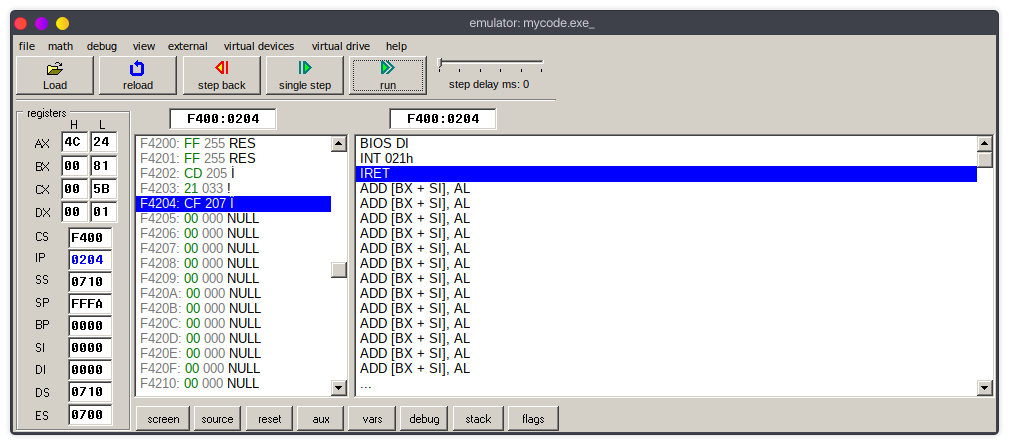
\includegraphics[width=0.90\textwidth]{img/p16/ss1.png}
	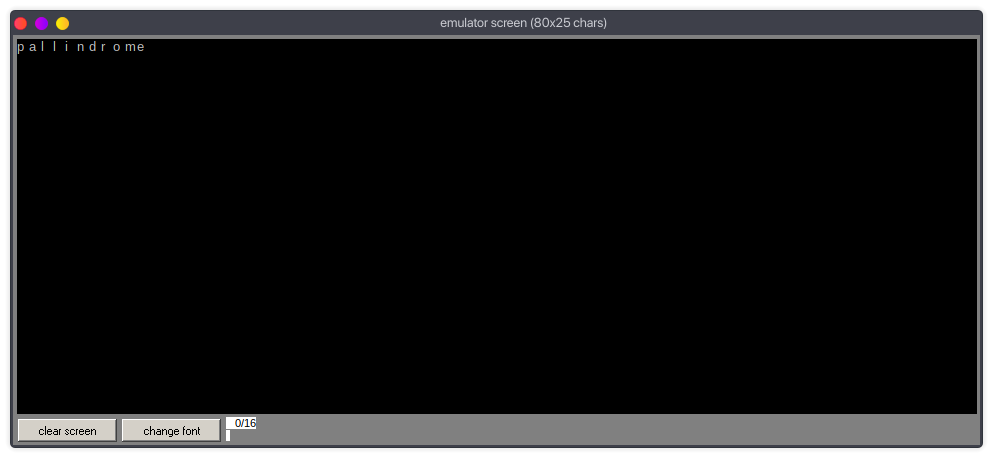
\includegraphics[width=0.90\textwidth]{img/p16/ss2.png}\\
    Output for 81H\\

    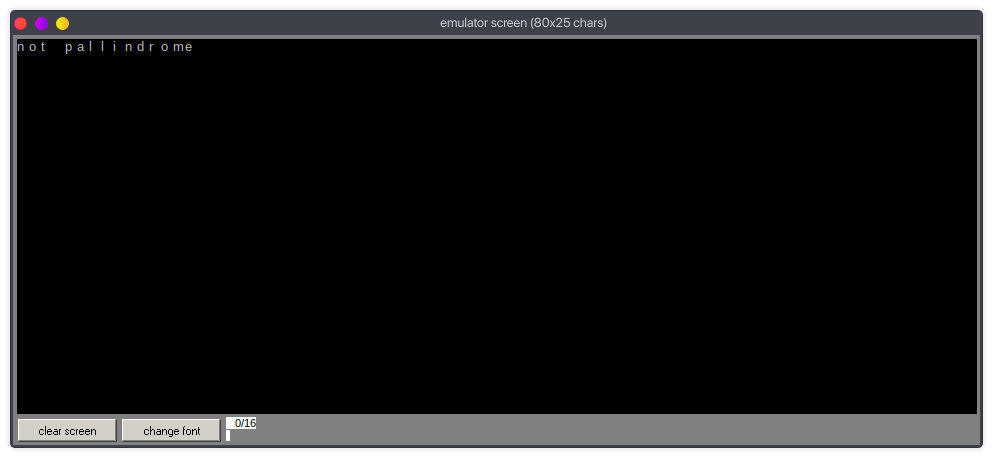
\includegraphics[width=0.90\textwidth]{img/p16/ss3.png}\\
    Output for 82H\\
\end{center}

\subsection{Result}
The number was checked to be pallindrome in its binary representation

